% ID = 35
%%%%%%%%%%%%%%%%%%%%%%% file template.tex %%%%%%%%%%%%%%%%%%%%%%%%%
%
% This is a general template file for the LaTeX package SVJour3
% for Springer journals.          Springer Heidelberg 2010/09/16
%
% Copy it to a new file with a new name and use it as the basis
% for your article. Delete % signs as needed.
%
% This template includes a few options for different layouts and
% content for various journals. Please consult a previous issue of
% your journal as needed.
%
%%%%%%%%%%%%%%%%%%%%%%%%%%%%%%%%%%%%%%%%%%%%%%%%%%%%%%%%%%%%%%%%%%%
%
% First comes an example EPS file -- just ignore it and
% proceed on the \documentclass line
% your LaTeX will extract the file if required
% \begin{filecontents*}{example.eps}
% %!PS-Adobe-3.0 EPSF-3.0
% %%BoundingBox: 19 19 221 221
% %%CreationDate: Mon Sep 29 1997
% %%Creator: programmed by hand (JK)
% %%EndComments
% gsave
% newpath
%   20 20 moveto
%   20 220 lineto
%   220 220 lineto
%   220 20 lineto
% closepath
% 2 setlinewidth
% gsave
%   .4 setgray fill
% grestore
% stroke
% grestore
% \end{filecontents*}
%
\RequirePackage{fix-cm}
%
%\documentclass{svjour3}                     % onecolumn (standard format)
%\documentclass[smallcondensed]{svjour3}     % onecolumn (ditto)
\documentclass[smallextended]{svjour3}       % onecolumn (second format)
%\documentclass[twocolumn]{svjour3}          % twocolumn
\usepackage[cp1250]{inputenc}
%\usepackage[polish]{babel}
%\usepackage{polski}
%\usepackage{graphicx}
%\usepackage{amsthm}
\usepackage{amsmath}
\usepackage{amsfonts} %potrzebne do \mathbb{S}
\usepackage{overpic} %napisy na obrazkach
\usepackage{color}
%\usepackage[table]{xcolor}
%\usepackage{colortbl}
\usepackage{hhline}
\usepackage{dcolumn}
\usepackage{longtable}
\usepackage{fancyhdr}
\usepackage{subfig}
\usepackage{wrapfig}
\usepackage{here}
\usepackage{bm}
\usepackage{pbox}
\usepackage{booktabs}
\usepackage{ctable}
\usepackage{caption}
\usepackage{multirow}
\usepackage{color}
\def\red#1{{\color{red}{#1}\color{black}}}
\pagestyle{fancy}
\fancyhf{}
% numery stron: lewa do lewego (marginesu), prawa do prawego
\fancyhead[LE,RO]{\textbf{\thepage}}
% prawa pagina: zawarto�� \rightmark do lewego, wewn�trznego (marginesu)
\fancyhead[LO]{\small\sffamily \nouppercase{\rightmark}}
% lewa pagina: zawarto�� \leftmark do prawego, wewn�trznego (marginesu)
\fancyhead[RE]{\small\sffamily \nouppercase{\leftmark}}
% kreski oddzielaj�ce paginy (g�rn� i doln�):
\renewcommand{\headrulewidth}{0.4pt}
\renewcommand{\footrulewidth}{0.0pt}
\newcommand{\otoprule}{\midrule
[\heavyrulewidth]}\newtheorem{tw}{Theorem}
%\newtheorem{lemma}{Lemma}[section]
\newtheorem{df}{Definition}
\newtheorem{rmk}{Remark}

\smartqed  % flush right qed marks, e.g. at end of proof
%
\usepackage{graphicx}
%\usepackage{geometry}
%\geometry{tmargin=5cm,bmargin=4cm,lmargin=3cm,rmargin=3cm}
% \usepackage{mathptmx}      % use Times fonts if available on your TeX system
%
% insert here the call for the packages your document requires
%\usepackage{latexsym}
% etc.
%
% please place your own definitions here and don't use \def but
% \newcommand{}{}
%
% Insert the name of "your journal" with
% \journalname{myjournal}
%
\begin{document}

\title{Maintenance management of mining belt conveyor system based on data fusion and advanced analytics}
%\subtitle{Do you have a subtitle?\\ If so, write it here}

\author{Pawel Stefaniak$^{1}$\ and Jacek Wodecki$^{1}$\ and Radoslaw Zimroz$^{1}$}

%\authorrunning{Short form of author list} % if too long for running head

\institute{$^1$Diagnostics and Vibro-Acoustics Science Laboratory, Wroclaw University of Science and Technology Na Grobli 15, 50-421 Wroclaw, Poland}

% \institute{$^2$Diagnostics and Vibro-Acoustics Science Laboratory, Wroclaw University of Technology, Na Grobli 15, 50-421 Wroclaw, Poland}
\date{Received: date / Accepted: date}
% The correct dates will be entered by the editor

\maketitle

\begin{abstract}
Belt conveyor network is an important transportation form used in underground copper ore mines. Effective maintenance of this infrastructure is critical - serious failure of single conveyor might stop operation of several conveyors connected in series and finally might affect production volume. To achieve expected reliability one should use appropriate tools for supporting maintenance management and decision making process. Nowadays predictive maintenance seems to be the most powerful approach for industrial applications. Deep understanding design and operational factors, knowledge about of repairs (number, type, reasons...) and finally acquisition and processing of appropriate physical variables might provide suitable information for maintenance staff. However, mining industry, especially underground mine is a specific kind of factory. Harsh environmental conditions (high humidity, temperature, dust, etc.), varying load, specific damage scenarios make practical implementation of predictive maintenance difficult. Also scale of transportation system plays an important role: $>80$ conveyors with different configurations (1-4 drives), diversity of dimensions (short vs. long conveyors), locations (environmental issues, operation on the slope) etc. All these facts required special approach based on diagnostic data acquisition, necessary processing and context-based reasoning. In the paper we will discuss details related to development of analytical IT-based environment integrating data from many different sources and procedures supporting decision making process. We will propose the concept of Decision Support System for maintenance of conveyors system. Because of the multidimensional nature of diagnostic data and diversified technical configurations of the facilities, it was necessary to develop and implement multivariate analytical models including data fusion and artificial intelligence techniques. Consequently, it allows to avoid failures, support scheduling repairs and finally provides reduction of repairs costs and production losses related to breakdowns.

\keywords{belt conveyor \and diagnostics \and data mining \and maintenance management support system}

\end{abstract}
\section{Introduction}
Belt conveyor transport in Polish copper ore mining industry is a main component of technological line responsible for majority of horizontal haulage of ore. 
In the regarded mine there are over 80 exploited conveyors routes, of total length exceeding 50 kilometers, distributed spatially in five main areas of the mine. Scheme of conveyor network is presented in (Fig. \ref{fig: f1}a). Achieving presumed overall efficiency of the mine is strongly dependent on used haulage automation and reliability of the conveyors. Harsh mining conditions of operation (high external load, complicated environmental parameters: high temperature and humidity, dust and air salinity) has a direct effect on  reliability of conveyors \cite{Kacprzak2011}. Beside the diversity of failure types and forms of wear of their components, failures regarding elements of driving units are critical from the conveyor availability point of view (Fig. \ref{fig: f1}b).
\begin{figure}[ht!]
\centering
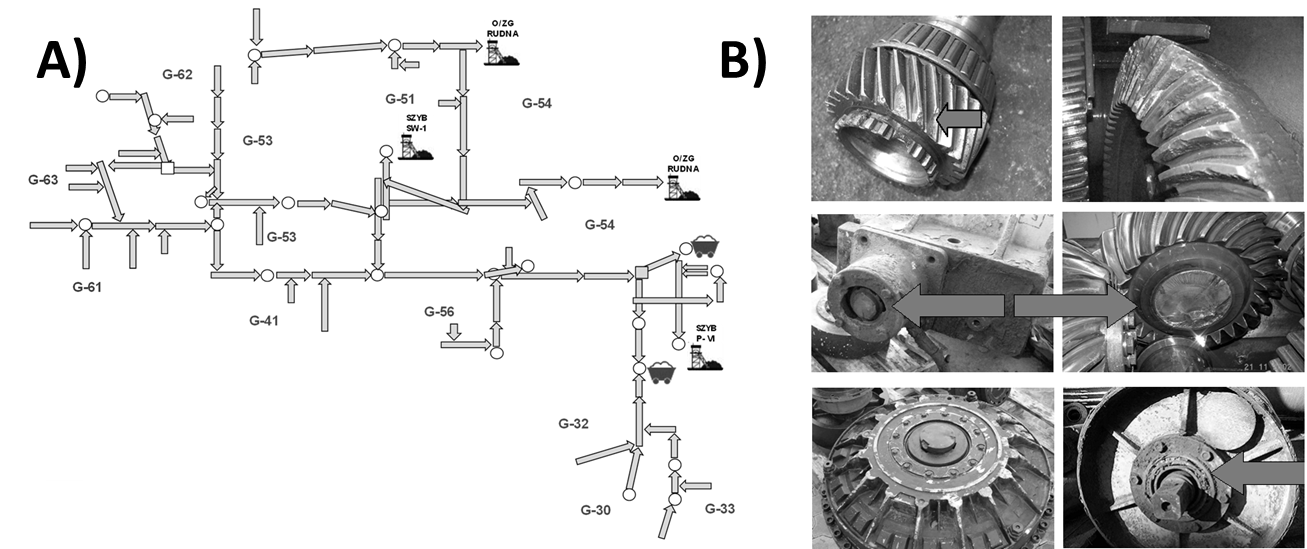
\includegraphics[width = \textwidth]{Wykresy/Fig_1}
\caption{a) Conveyor transportation network of Polkowice-Sieroszowice Mine, b) examples of critical failures of components in driving units (from the top: gear damage, ruptured shaft of gearbox, ruptured shaft of the coupling)}
\label{fig: f1}
\end{figure}
In regarded mine annual costs of driving units repairs make about $28-37$\%  of total costs of conveyors  maintenance. Conducted failure analysis \cite{Zimroz2009} shows that utilized planned preventive strategy of exploitation is not an optimal solution for conveyor haulage from the view point of maintenance cost minimization and conveyor availability maximization. To achieve full exploitation potential of regarded machine park requires constant availability of information regarding technical, organizational and economical aspects \cite{Levitt2009,Lodewijks2004,Loska2013,Loska2012}. To be able to do that, it is important to constantly log the emergency events, as well as to perform online monitoring of technical condition and following exploitation indicators being real support for staff as a decision making aid \cite{Dabrowski2015,Drozyner2007,Galar2012,Kazmierczak1998}.
In this paper we present DiagManager, a maintenance management support system for network of belt conveyors, which is based on data fusion distributed amongst different databases \cite{StefaniakZimroz2014,Stefaniak2012}. Periodic tracking the diagnostic features and indicators variability might allow for estimation of remaining useful life (RUL) of technical objects and identification of objects indicating high risk of failure. It is useful e.g. for optimal scheduling of maintenance and repair actions. Early detection of faults and abnormalities in time helps to prevent complete failure in advance. It also contributes to reduction of maintenance cost and production losses through accidental events. Basic functionality of DiagManager system is presented in Fig. \ref{fig: f2}.
\begin{figure}[ht!]
\centering
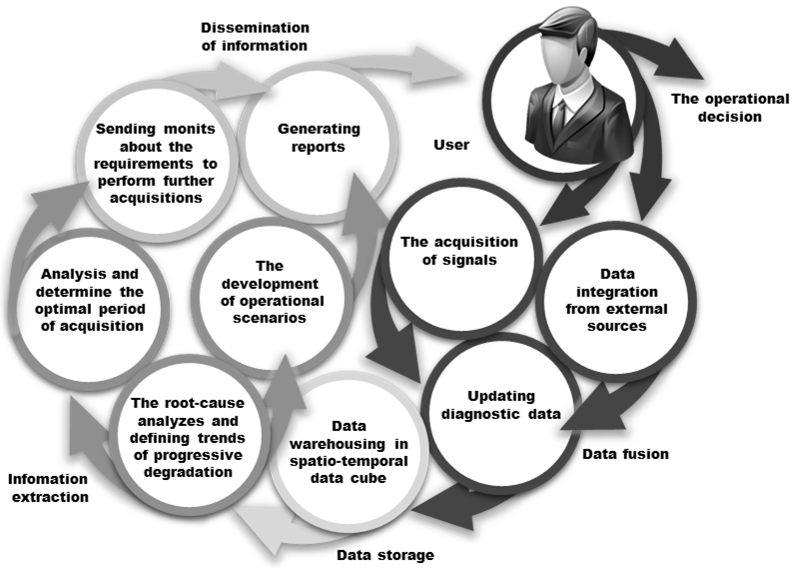
\includegraphics[width = 0.75\textwidth]{Wykresy/Fig_2}
\caption{Main functionality of management support system}
\label{fig: f2}
\end{figure}
\section{Functional scheme of management support system for conveyor transport maintenance and exploitation}
Investigated maintenance management support system is based on GIS platform. It is the response for identified information demands by management staff. The idea of system functionality is basically data integration from different sources (data acquisition, SAP-PM, technical and motion documentation, etc.) and fusion of information, which allows system to provide potential exploitation suggestions. Whole functionality is contained in system modules. Structural scheme of the system is presented in Fig.\ref{fig: f3}.
\begin{figure}[ht!]
\centering
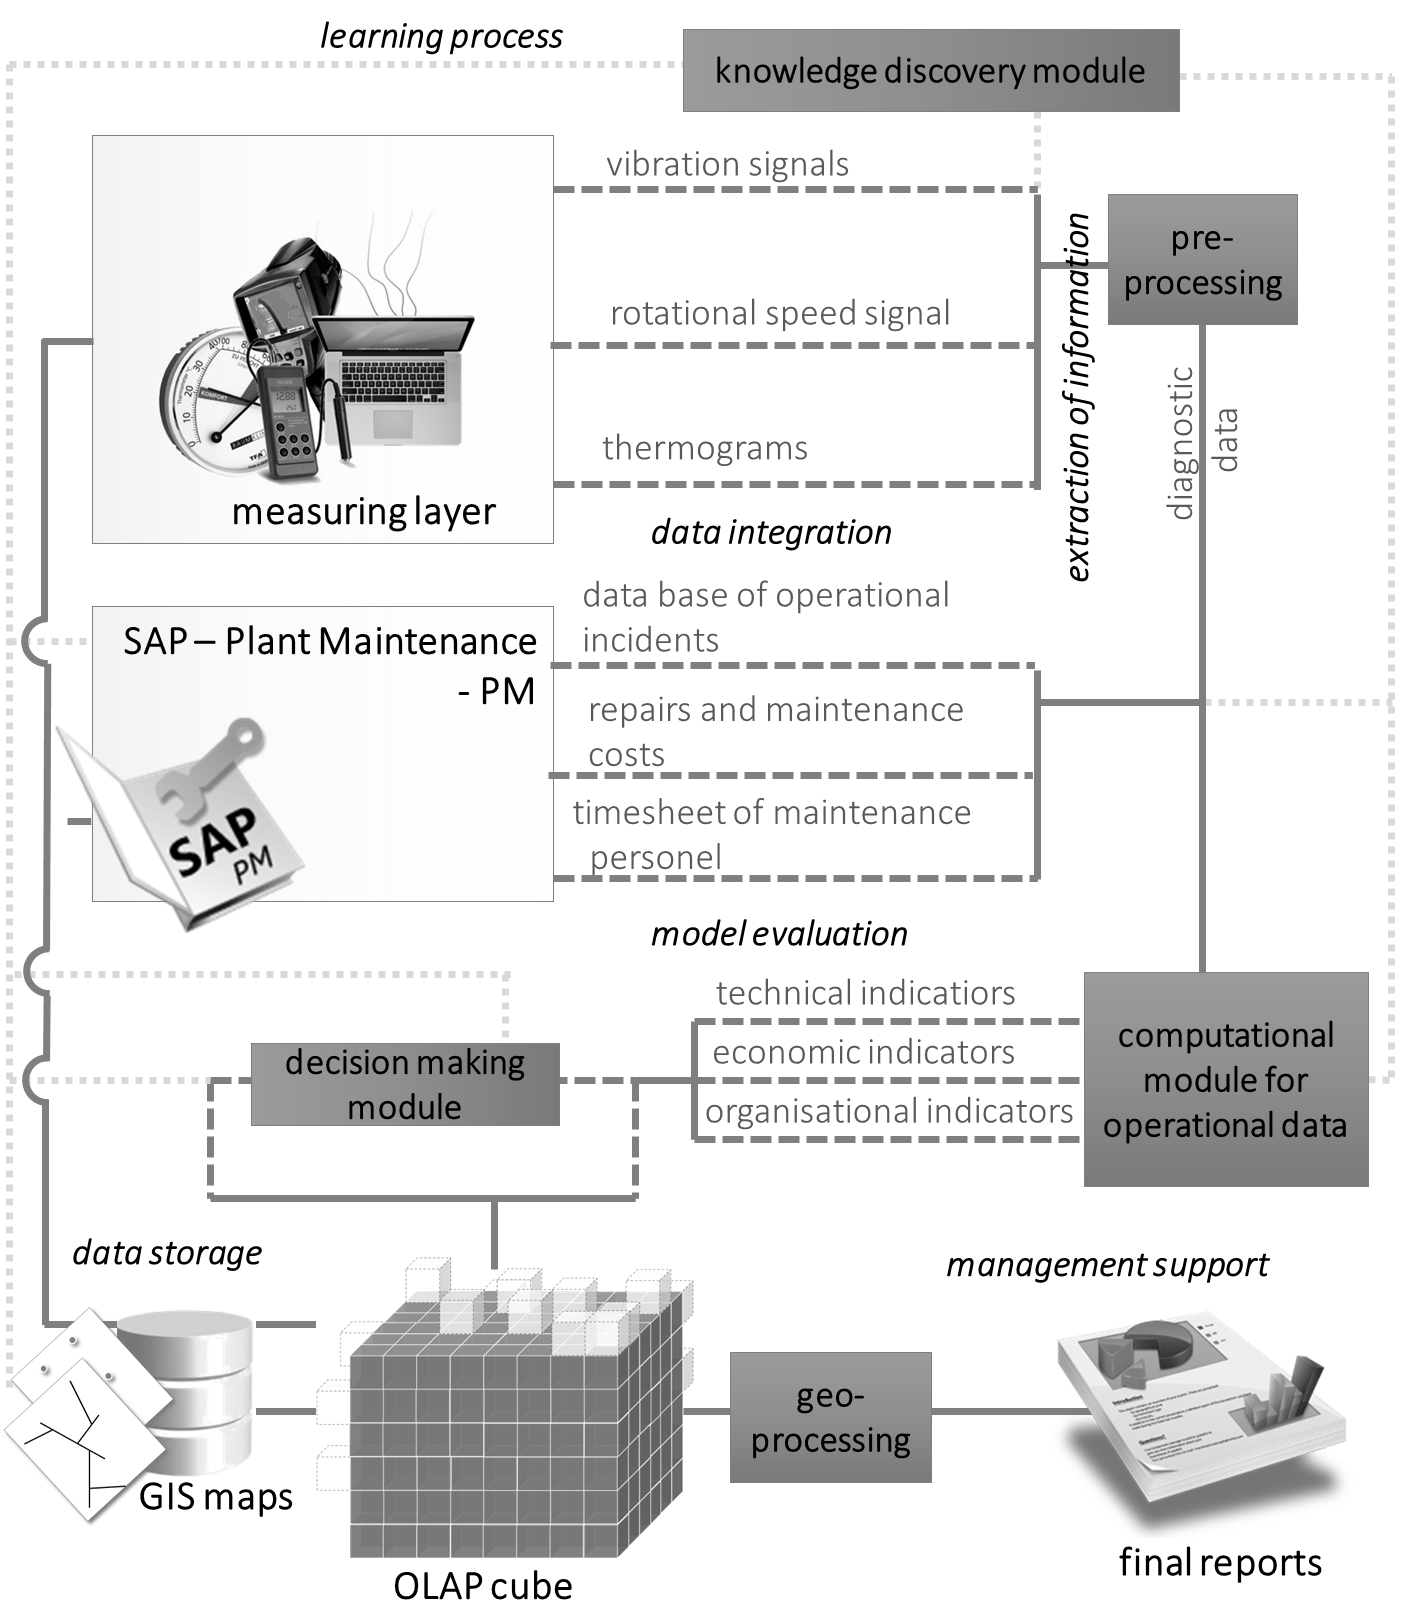
\includegraphics[width = 0.65\textwidth]{Wykresy/Fig_3}
\caption{Structure of CMMS-class DiagManager system for conveyors}
\label{fig: f3}
\end{figure} \par
Integral part of DiagManager system is mobile module of diagnostic data acquisition. It consists of two layers. First layer is responsible for control and measurement functionality of acquisition module and it is in practise a laptop computer with dedicated software. Second layer is the actual measurement hardware: three  accelerometers mounted on the housing of the gearbox, and the tachometer probe. Tachometer probe measures rotational speed of input shaft of gearbox, which is needed for determining external load of conveyor. This on the other hand is dependent on the amount of ore transported on the belt. Vibration measurement is complemented by thermograms of gearbox housing. Algorithms developed for diagnostic signal processing validate measured data for their quality and completeness, and after that they extract from signal spectrum diagnostic features, that indicate technical state of rotating elements of gearbox like shafts, gears and bearings.\par
Single measurement of diagnostic data lasts 60 seconds. Schedule of next diagnostic inspections depends on the results of diagnosis of elements state from last measurement session \cite{Stefaniak2014,Stefaniak2016}. 
Simultaneously such system should records exploitation events, costs and duration of maintenance and repair actions. This data is then processed by the algorithms implemented in computational module, calculating so called exploitation indicators. They take form of simple statistics or are produced by more algorithmically complicated procedures. List of defined indicators is presented in Tab. 1.
\begin{figure}[ht!]
\begin{flushleft}{\normalsize Tab. 1: List of exploitation indicators used in the process of supporting the management of conveyor network exploitation}\end{flushleft}
\centering
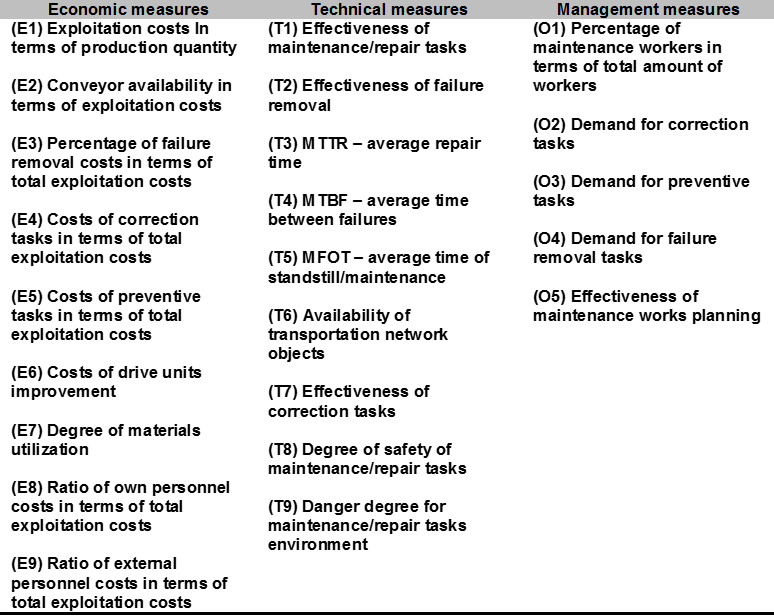
\includegraphics[width = 0.7\textwidth]{Wykresy/tab2.png}
%\caption{List of exploitation indicators used in the process of supporting the management of conveyor network exploitation}
\label{tab: t1}
\end{figure} \par
The decision module is responsible for interpretation of registered diagnostic data and exploitation indicators, and basing on them it presents suggestions regarding exploitation decisions to the user. Reporting tools are heavily connected with this module. GIS platform provides the visualization of results of conducted measurements and analyses on many kinds of thematic maps, which strongly increases readability of reports for the transportation network. 
In general, further analysis of diagnostic data and exploitation indicators enables:
\begin{itemize}
\renewcommand{\labelitemi}{$\bullet$}
\item analysis of technical state of gearbox components based on monitored symptoms (Fig.\ref{fig: f4}a,b,c),
\item localizing critical objects (Fig.\ref{fig: f4}d),
\item assessment of quality and effectiveness of maintenance staff actions,
\item assessment of quality of conveyors / conveyor divisions.
\end{itemize}
\begin{figure}[ht!]
\centering
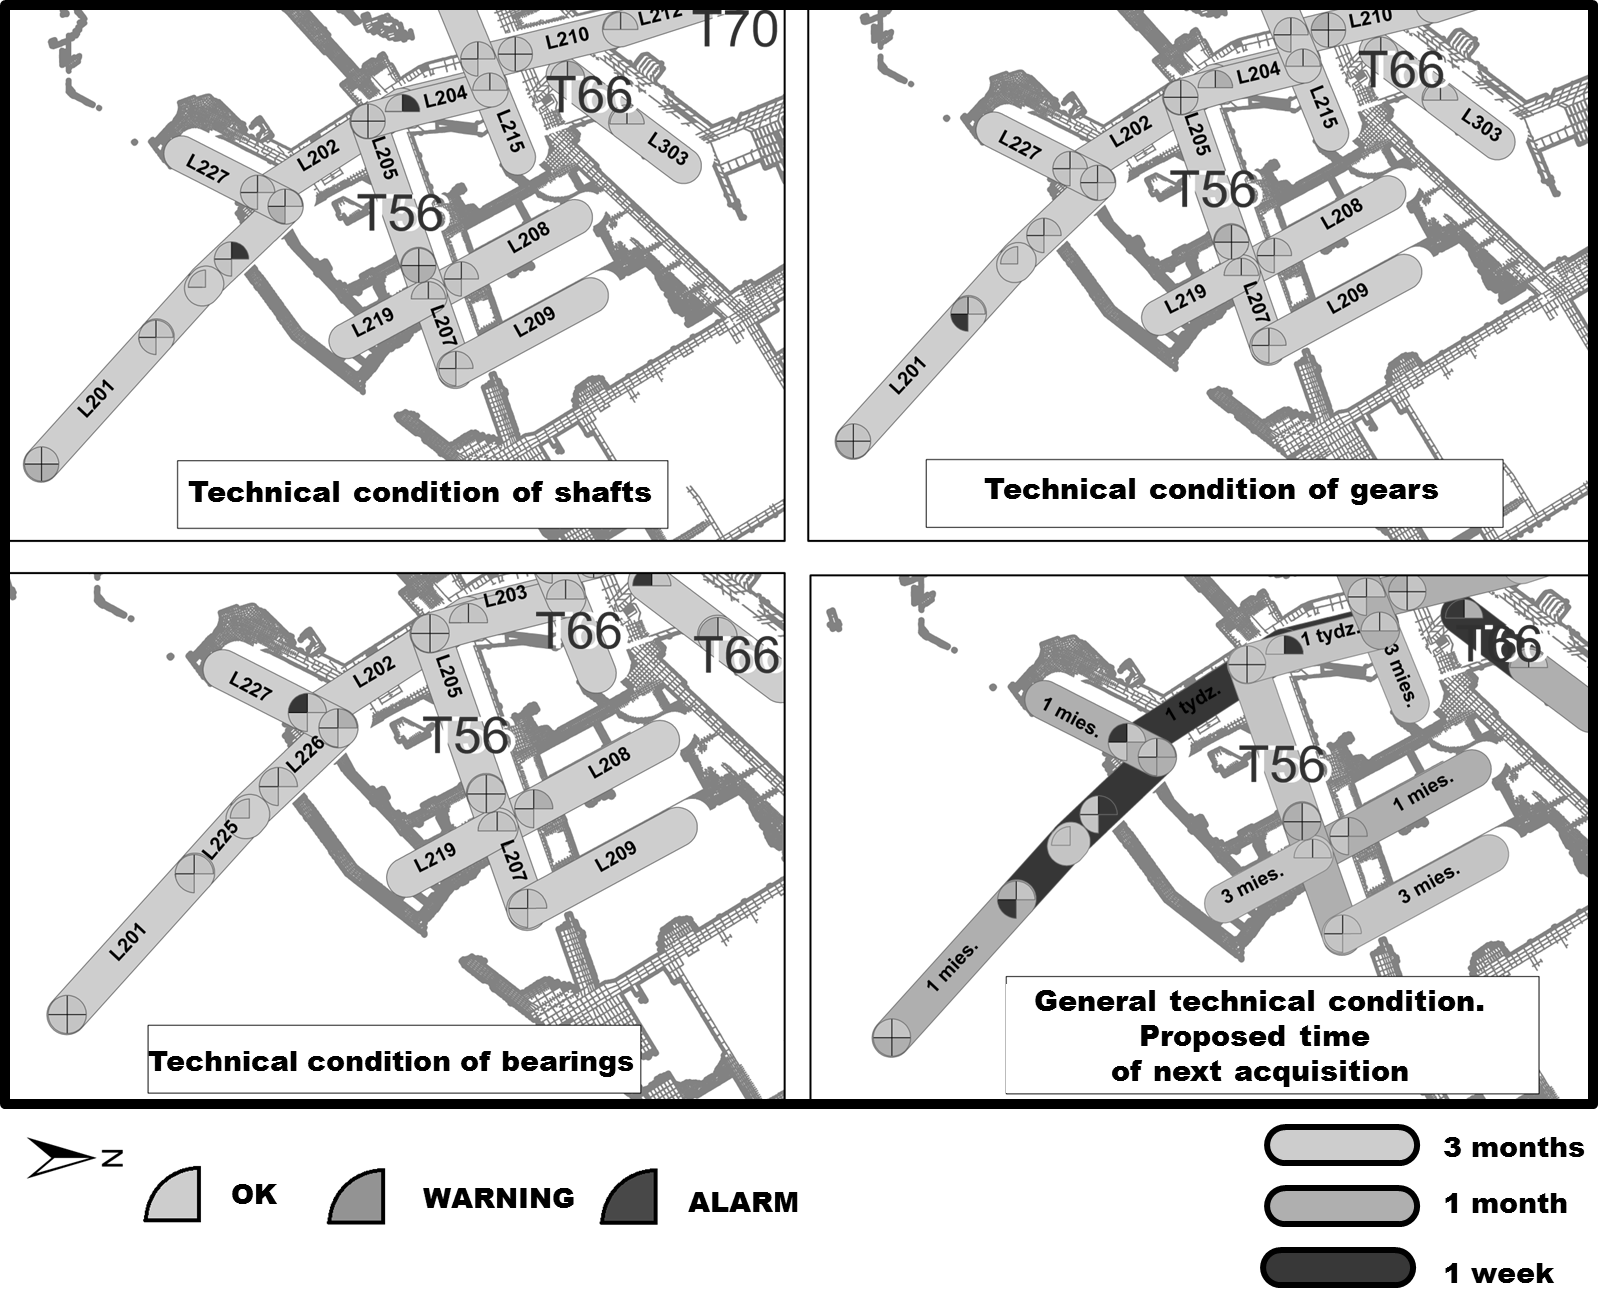
\includegraphics[width = 0.7\textwidth]{Wykresy/Fig_4}
\caption{Example of report for  conveyor division of Polkowice-Sieroszowice Mine concatenating general technical condition of conveyor gearboxes with distinction of their components and proposed scheduling for maintenance}
\label{fig: f4}
\end{figure} \par
\section{Decision making process}
Main tasks of decision module are:(a) constructing schedules for maintenance, (b) identification of objects for periodic diagnostic inspection, (c) making decisions connected to allowing conveyors to be exploited, (d) early identification of potential threats for safety of operation.

In case of diagnostic data constructing the decision algorithm required getting familiar with the data correlation structure, identifying threshold values for diagnostic features (Fig.\ref{fig: f5}a) dependent on external load \cite{Bartelmus2009,Stefaniak2014,Stefaniak2016,StefaniakZimroz2014,Zimroz2014}, formulating degradation model (Fig.\ref{fig: f5}b) and building the structure of artificial neural network for recognizing technical condition of gearbox components (Fig.\ref{fig: f5c}). Neural network diagnoses shafts, gears and bearings based on training set of data, assigning  to each of them one of three possible classes: ok (correct condition), warning (early phase of component wear), alarm (critical condition). Basing on this estimate overall condition is stated, which is worst of classes assigned to components of one gearbox by neural network.
\begin{figure}[ht!]
\centering
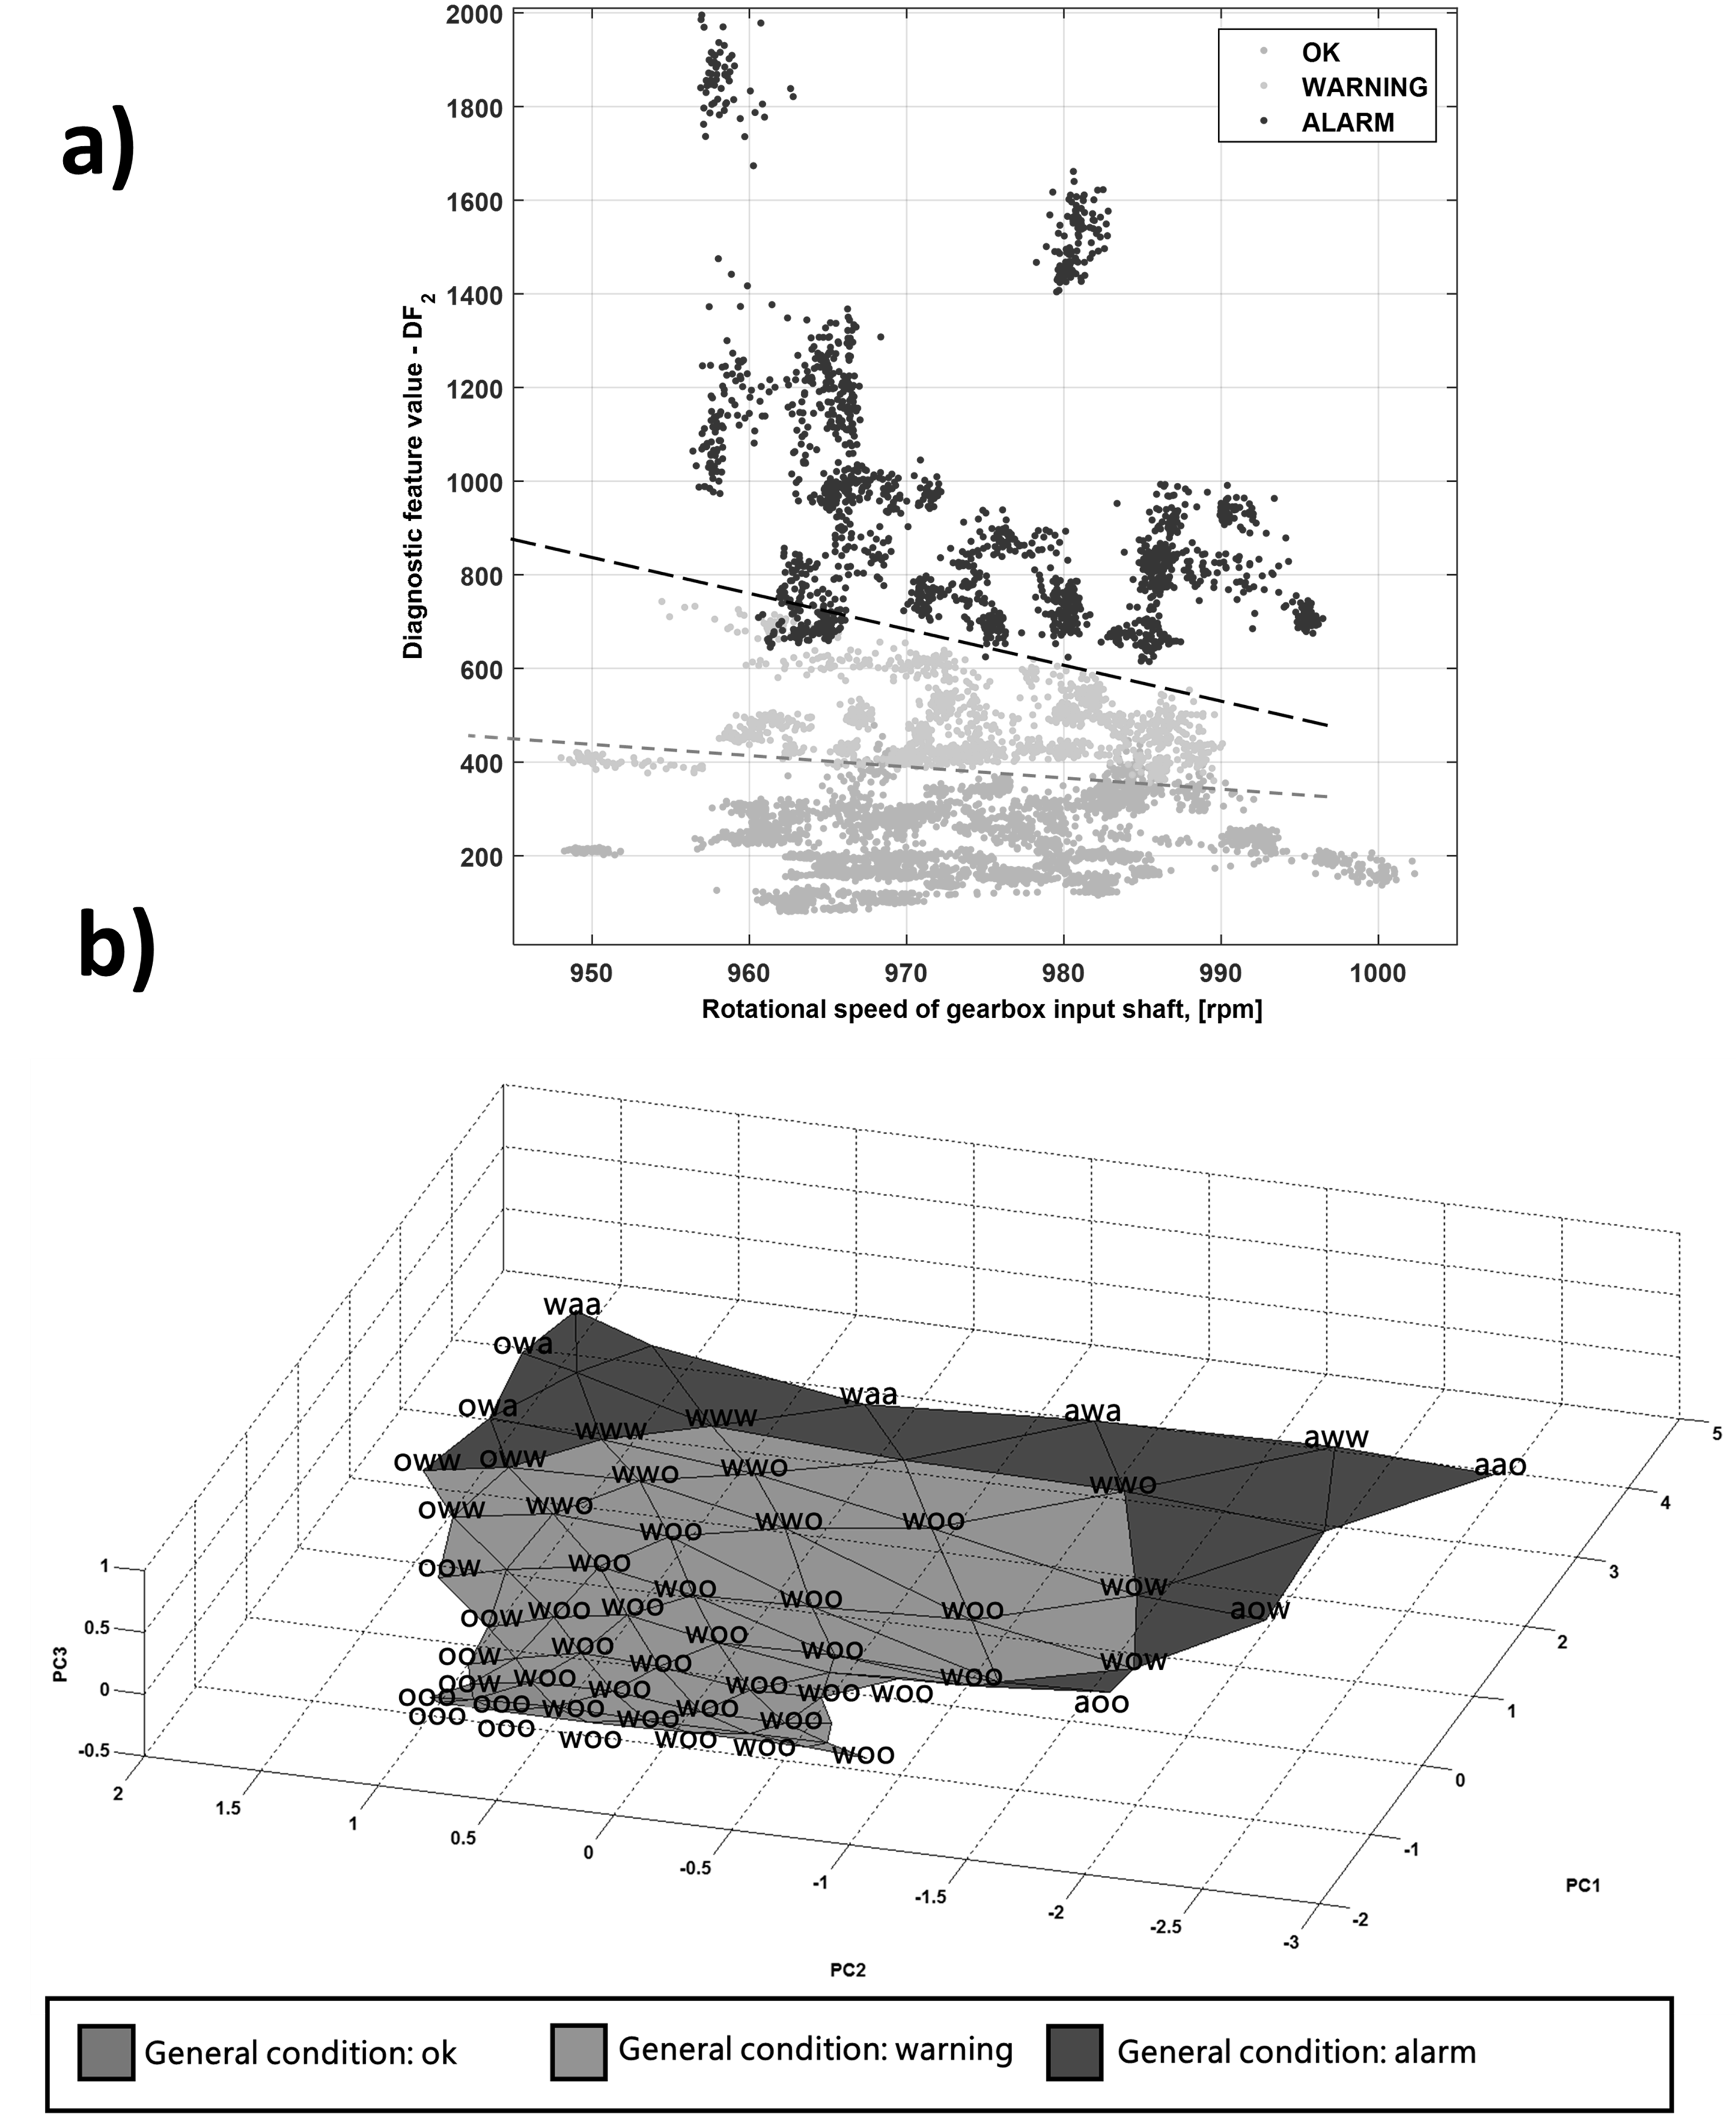
\includegraphics[width =0.7\textwidth]{Wykresy/Fig_5.png}
\caption{Process of diagnostic algorithm construction: a) recognition of correlation structure of diagnostic data and identification of threshold values (here the case of one feature), b) model construction for gearbox degradation process}
\label{fig: f5}
\end{figure}
\begin{figure}[ht!]
\centering
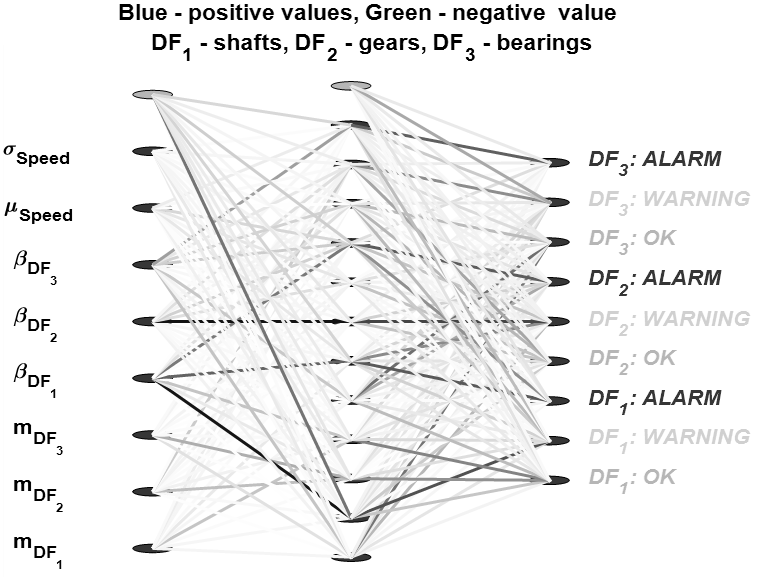
\includegraphics[width =0.6\textwidth]{Wykresy/Fig_5c.png}
\caption{Building a structure of neural network for condition recognition}
\label{fig: f5c}
\end{figure}
Additionally in decision making process exploitation indicators are taken into consideration (see Tab. 2). Those indicators are scaled with taximetric methods into the form of stimulants. Designed algorithm identifies objects with lower-than-expected values of indicators, and returns appropriate flags and exploitation suggestions. This way, basing on if-then-else-type decision objects are selected and maintenance schedule is planned. In similar way we define the schedule for diagnostic inspections or enabling the objects to operate. Exemplary formulae for calculating selected indicators along with the method of their interpretation is presented in the Tab. 2. \par

\begin{figure}[ht!]
\begin{flushleft}{\normalsize Tab. 2: Exemplary formulae for calculating selected indicators along with the method of their interpretation}\end{flushleft}
\centering
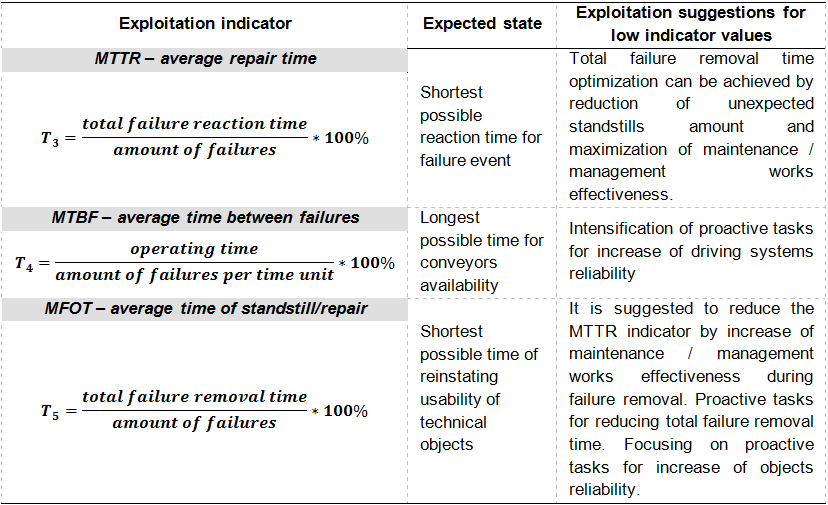
\includegraphics[width =0.7\textwidth]{Wykresy/tab.PNG}
\label{fig: f7}
\end{figure}



\begin{figure}[ht!]
\centering
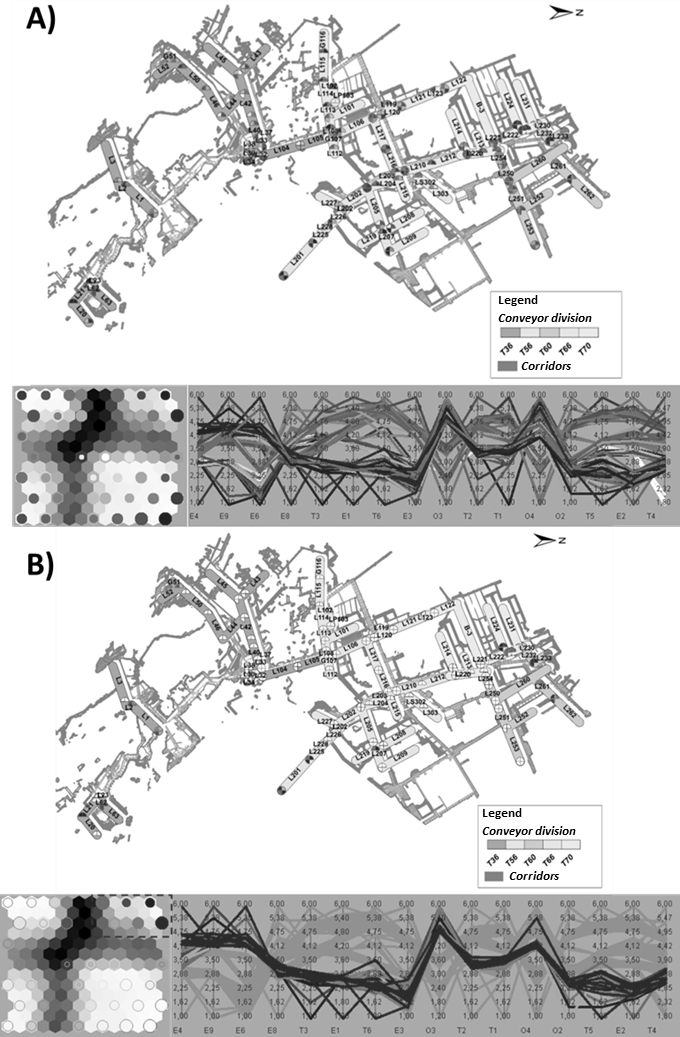
\includegraphics[width =0.8\textwidth]{Wykresy/Fig_6.png}
\caption{a) Example result of SOM clustering. Object with similar properties grouped up into clusters. Result of cluster analysis is presented on visualization components by appropriate colors, b) Selected red pattern of SOM clustering result presented on GIS-type map (top), on U-Matrix map (bottom left) and PCP chart (bottom right). Selection by marking red pattern on  U-Matrix map}
\label{fig: f6}
\end{figure}


Considering the amount of driving units of this transportation system (over 220) as well as the amount of defined exploitation indicators, it was necessary to propose a simple method for data exploration with the option of spatial presentation of results of the analysis. We implemented the algorithm based on self-organizing maps (SOM), allowing to identify objects of similar characteristics based on clustering of multidimensional data set of indicators. Thanks to that, we can recognize some unknown early regularities (especially in spatial context) related to exploitation process of this transportation network. To present the clustering results we use three visualization components: GIS-type map, PCP chart and U-Matrix map showing the projection of SOM. Patterns (classes) represented by individual groups of similar properties, group up in certain areas of the U-Matrix map and are also presented by appropriate colors (Fig. 7a). Black hexagons represent borders of classes. Application interface allows for easy interaction between the user and visualization components, which allows for selection of particular cluster on the visualization component with drag-and-drop method. Fig. 7b presents example result of red pattern selection. Implementation process of selection result from Fig. 7b is very simple and intuitive. GIS-type map presents the localization of objects qualified for red class, and PCP chart illustrates the variability of exploitation scores of those objects. Red pattern indicates the objects of the highest exploitation costs in relation to production volume (E1) and greatest percentage ratio of costs wasted on failure removal in relation to overall exploitation costs. (E3). Moreover, the lowest degree of conveyors availability was observed (E2, T5). Exploitation suggestions provided by DiagManager system for red pattern is intensification of correction and prevention actions and focusing on increased effectiveness of failure removal. 

\section{Summary}
Maintenance management of conveyors network in underground copper ore mine requires dedicated computerized system for management staff because of many reasons (amount of technical objects, the spatial aspect, different design features, exploitation conditions etc.). Functional and informational needs for IT system design have been identified. According to them, we present the overview of such data fusion oriented system. Acquiring data from the acquisition system, integration of data distributed among different database systems and development of proper analytical models, reasoning criteria and reporting tools allow for constant monitoring of transportation network and maintenance staff in technical, economical and organizational aspects. In the paper we present the scheme and functional idea of such system by example of selected KGHM mine. System supports the transportation network exploitation staff in the matter of: (a) scheduling maintenance actions, (b) identification of objects for periodic diagnostic inspection, (c) making decisions regarding admitting the conveyors to operate, (d) early recognition of potential threats for work safety.

\textbf{Acknowledgements}\par
This work is supported by the statutory grant No. B50137 (P. Stefaniak).

\begin{thebibliography}{}

\bibitem{Bartelmus2009} Bartelmus W., Zimroz R.,\emph{A new feature for monitoring the condition of gearboxes in non-stationary operating conditions }, 2009, Mechanical Systems and Signal Processing. Vol. 23 No 5, pp. 1528-1534.

\bibitem{Dabrowski2015} Dabrowski M.,\emph{The supporting of exploitation and maintenance management within networked technical systems}, 2015, Management Systems in Production Engineering.Vol. 5 No 2, pp. 81-87.

\bibitem{Drozyner2007} Drozyner P., Mikolajczak P., \emph{Assessment of the effectiveness of machine and device operation}, 2007, Eksploatacja i Niezawodnosc – Maintenance and Reliability. Vol. 3 No 35, pp. 72-75.

\bibitem{Galar2012}Galar D., Gustafson A.,Tormos B., Berges L.,\emph{Maintenance decision making based on different types of data fusion}, 2012, Eksploatacja i Niezawodnosc – Maintenance and Reliability. Vol. 14 No 2, pp. 135-144.

\bibitem{Kacprzak2011} Kacprzak M., Kulinowski P., Wedrychowicz D.,\emph{Computerized information system used for management of mining belt conveyors operation}, 2011, Eksploatacja i Niezawodnosc – Maintenance and Reliability. Vol. 50 No 2, pp. 81-93.

\bibitem{Kazmierczak1998} Kazmierczak J., Kristovic D.,\emph{Some aspects of computer supported maintenance management},1998,Proceedings of Euromaintenance 98.Dubrovnik.

\bibitem{Levitt2009} Levitt J ,\emph{The handbook of maintenance management (second edition)}, 2009, New York: Industrial Press Inc.

\bibitem{Lodewijks2004} Lodewijks G.,\emph{Strategies for automated maintenance of belt conveyor systems}, 2004, BulkSolids. Vol. 24 No 1, pp. 16-22.

\bibitem{Loska2013} Loska A.,\emph{Exploitation assessment of selected technical objects using taxonomic methods}, 2013, Maintenance and Reliability. Vol. 15 No 1, pp. 1-8.

\bibitem{Loska2012} Loska A.,\emph{Remarks about modelling of maintenance processes with the use of scenario techniques}, 2012, Maintenance and Reliability. Vol. 14 No 2, pp. 92-98.

\bibitem{Sawicki} Sawicki M., Zimroz R., Wylomanska, Obuchowski J., Stefaniak P., Zak G.,\emph{An Automatic Procedure for Multidimensional Temperature Signal Analysis of a SCADA System with Application to Belt Conveyor Components}, Procedia Earth and Planetary Science 15, 2015, pp. 781-790.

\bibitem{Stefaniak2014} Stefaniak P.,  Wylomanska A.,  Obuchowski J., Zimroz  R.,\emph{Procedures for decision thresholds finding in maintenance management of  belt conveyor  system - statistical modeling of diagnostic data}, 2015, Proceedings of the 12th International Symposium Continuous Surface Mining - Aachen 2014. Springer, pp. 391-402.

\bibitem{Stefaniak2016} Stefaniak P., Wylomanska A., Zimroz R., Bartelmus W., Hardygora M.,\emph{ Diagnostic features modeling for decision boundaries calculation for maintenance of gearboxes used in belt conveyor system}, 2016, Advances in Condition Monitoring of Machinery in Non-Stationary Operations. Proceedings of the Fourth International Conference on Condition Monitoring of Machinery in Non-Stationary Operations, CMMNO'2014, Lyon, Springer, pp. 251-263.

\bibitem{StefaniakZimroz2014} Stefaniak P., Zimroz R., Bartelmus W., Hardygora M.,\emph{Computerised decision-making support system based on data fusion for machinery system's management and maintenance}, 2014, Applied Mechanics and Materials. Vol. 683, pp. 108-113.

\bibitem{Stefaniak2012} Stefaniak P., Zimroz R., Krol R., Gorniak-Zimroz J., Bartelmus W., Hardygora M.,\emph{Some remarks on using condition monitoring for spatially distributed mechanical system belt conveyor network in underground mine - A Case Study}, 2012, Condition Monitoring of Machinery in Non-Stationary Operations. Springer, pp. 497-507, doi:10.1007/978-3-642-28768-8\_51.

\bibitem{Tewari1991} Tewari P.C., Singh I.P, Khare M.K.,\emph{Reliability analysis of a conveyor belt system, with only one server, subject to failures and idleness after repair}, 1991, Microelectronics Reliability. Vol. 31 No 5, pp. 823-826.

\bibitem{Zimroz2009} Zimroz R., Krol R.,\emph{Failure analysis of belt conveyor systems for condition monitoring purposes}, 2009, Prace Naukowe Instytutu G{\'o}rnictwa Politechniki Wroc{\l}awskiej. Studia i Materia{\l}y. Vol. 128 No 36, pp. 255-270.

\bibitem{Zimroz2014} Zimroz R., Stefaniak P., Bartelmus W. Hardygora M.,\emph{Novel techniques of diagnostic data processing for belt conveyor maintenance}, 2015, Proceedings of the 12th International Symposium Continuous Surface Mining - Aachen 2014. Springer, pp. 31-40.




\end{thebibliography}

\end{document}
% end of file template.tex
